\subsubsection{solución}
\begin{itemize}
\item Considerando un periodo de muestreo de $ T_s = 1 $ y utilizando el método de discretización [...] punto decimal hasta $T_s = 0,0001$).
\end{itemize}

Empezaremos por encontrar la ecuación en diferencias. Para esto tendremos que utilizar la definición que nos permite transformar de una ecuación diferencial a una en diferencias:

\begin{equation}
\frac{dy}{dx}=\frac{y(t)-y(t-T_s)}{T_s}
\end{equation}

\noindent e igualmente usaremos la que nos permite pasar de una diferencial de segundo grado a su equivalente en diferencias:

\begin{equation}
\frac{d^2y}{dt^2)}=\frac{y(t)-2y(t-T_s)+y(t-2T_s}{T_s^2}
\end{equation}

\noindent Tras sustituir ambas definiciones llegamos a:

\begin{equation}
\frac{V_c(t)-2V_c(t-T_s)+V_c(t-2T_s)}{T_s^2}+\frac{R}{L}\frac{V_c(t)-V_c(t-T_s)}{T_s}+\frac{1}{LC}V_c(t)=\frac{1}{LC}V_g(t)
\end{equation}

\noindent Aplicamos las equivalencias que nos dieron al inicio de la práctica $\frac{R}{L}=5$, $\frac{1}{LC}=5$, $V_c(t)=y(t)$ y $V_g(t)=x(t)$

\begin{equation}
\frac{y(t)-2y(t-T_s)+y(t-2T_s)}{T_s^2}+\frac{y(t)-y(t-T_s)}{T_s}+5y(t)=5x(t)
\end{equation}

\noindent \textbf{Salida con $T_s=1$}

\begin{figure}[H]
\centering
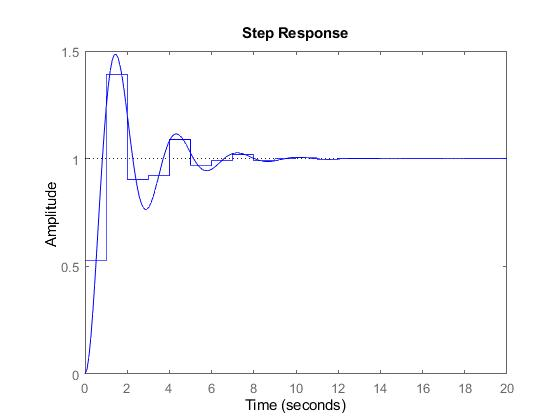
\includegraphics[width=0.7\linewidth]{SalidaTs1}
\caption{Salida con $T_s=1$}
\label{fig:salidaTs1}
\end{figure}

\noindent \textbf{Salida con $T_s=0,0001$}

\begin{figure}[H]
\centering
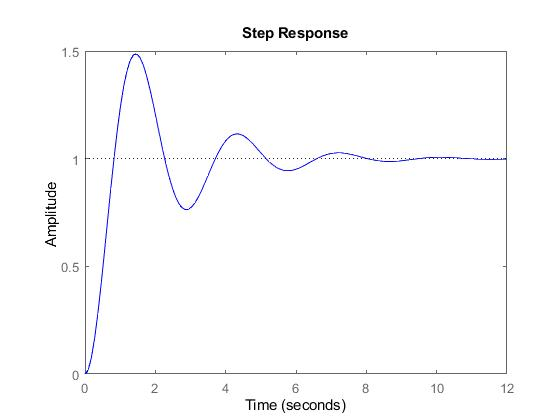
\includegraphics[width=0.7\linewidth]{SalidaTs00001}
\caption{Salida con $T_s=0,0001$}
\label{fig:salidaTs01}
\end{figure}

Para la obtención de las gráficas anteriores se usaron los siguientes comandos de Matlab:

\begin{itemize}
\item Ts=1
\item Hs=tf([5],[1 1 5])
\item Hz=c2d(Hs,Ts,'foh')
\item step(Hs,'-',Hz,'-')
\end{itemize}


Como podemos concluir de observar ambas gráficas, la importancia de $T_s$ radica en que mientras más se acerque su valor a cero mejor será la aproximación de la solución de ecuaciones por diferencias a la solución de la ecuación en tiempo continuo. Esto mismo lo podemos ver al hacer $T_s=0.0001$ parece que las gráficas se sobreponen, mientras que en $T_s=1$ se ve claramente la diferencia entre ambas gráficas. Cabe aclarar que la gráfica obtenida mediante la solución de diferencias finitas nunca va a ser la misma que la de tiempo continuo sin importar cuanto se disminuya $T_s$

\begin{itemize}
	\item Obtenga la función de transferencia del sistema de tiempo continuo.
	\item Utilizando $ T_s = 1 $:
\end{itemize}

\begin{equation}
	H(s)=\frac{Y(s)}{X(s)}=\frac{5}{(s^2+s+5)}
\end{equation}


\textbf{A)} Obtenga la función de transferencia de tiempo discreto de la ecuación en diferencias que resultó en	el punto anterior.

A partir de la ecuación obtenida en el ejercicio anterior

\begin{equation}
	\frac{y(t)-2y(t-T_s)+y(t-2T_s)}{T_s^2}+\frac{y(t)-y(t-T_s)}{T_s}+5y(t)=5x(t)
\end{equation}

Podemos llegar a que si $T_s=1$ nuestra ecuación por diferencias es la siguiente:



\begin{equation}
	\frac{0.5252z^2+1.231z+0.3053}{z^2 +0.6936x + 0.3679}
\end{equation}

Dicha ecuación es obtenida en Matlab tras usar los siguientes comandos.

\begin{itemize}
	\item Ts=1
	\item Hs=tf([5],[1 1 5])
	\item Hz=c2d(Hs,Ts,'foh')
\end{itemize}

\textbf{B)}  Obtenga la función de transferencia de tiempo discreto a partir de la función de transferencia de tiempo continuo del sistema utilizando un diferenciador discreto, ¿cómo son las funciones de transferencia obtenidas en este punto y el anterior? ¿qué puede concluir?

Como ya habíamos mencionado antes, la función de transferencia en tiempo discreto utilizando un diferenciador discreto es la siguiente:

\begin{equation}
	\frac{0.5252z^2+1.231z+0.3053}{z^2 +0.6936x + 0.3679}
\end{equation}

La comparación entre la obtención de la función de transferencia con y sin diferenciador se ve en las gráficas de la siguiente pregunta. Lo que se puede observar es que mediante el uso del diferenciador, la ecuación y su gráfica se acercan más a la ecuación y gráfica de la respuesta en tiempo continuo, es decir, la presencia del diferenciador hace más exacta la aproximación en tiempo discreto.